\documentclass[11pt]{article}
\usepackage{amsmath,amsthm,amssymb,fullpage,graphicx,hyperref,listings}
\usepackage{listings,color,setspace}
\author{Andy Reagan}
\title{Math 337 TEST 1}

     \def\NN{\mathbb{N} }
     \def\ZZ{\mathbb{Z} }
     \def\QQ{\mathbb{Q} }
     \def\RR{\mathbb{R} }
     \def\CC{\mathbb{C} }
     \def\f{\frac }
     \def\b{\begin }
     \def\e{\end }
     \def\Log{\text{Log} \,}
     \def\Re{\text{Re} \, }

\lstset{language=MATLAB,
basicstyle=\ttfamily\scriptsize\singlespacing,
keywordstyle=\color{blue},
stringstyle=\color{red},
commentstyle=\color{green},
morecomment=[l][\color{magenta}]{\#},
frame=L,
xleftmargin=\parindent,
%%numbers=left,                   %% where to put the line-numbers
%%numberstyle=\scriptsize,      %% the size of the fonts that are used for the line-numbers
%%stepnumber=1,                   %% the step between two line-numbers. If it is 1 each line will be numbered
numbersep=5pt,
breaklines=true,        %% sets automatic line breaking
breakatwhitespace=false,    %% sets if automatic breaks should only happen at whitespace
escapeinside={\%*}{*)} 
}


     \newcommand{\pdiff}[2]{\frac{\partial #1}{\partial #2}}
     \newcommand{\partialdiff}[2]{\frac{\partial #1}{\partial #2}}
     \newcommand{\pdiffsq}[2]{\frac{\partial^2 #1}{{\partial #2}^2}}
     \newcommand{\pdiffcu}[2]{\frac{\partial^3 #1}{{\partial #2}^3}}
     \newcommand{\pdiffhi}[3]{\frac{\partial^#3 #1}{{\partial #2}^#3}}
     \newcommand{\diff}[2]{\frac{{\rm d}#1}{{\rm d}#2}}
     \newcommand{\diffsq}[2]{\frac{{\rm d}^{2}#1}{{\rm d} {#2}^2}}
     \newcommand{\diffhi}[3]{\frac{{\rm d}^#3 #1}{{\rm d} {#2}^#3}}
     \newcommand{\tdiff}[2]{\mbox{d} #1/\mbox{d} #2}
     \newcommand{\tdiffsq}[2]{\mbox{d}^{2} #1/\mbox{d} {#2}^2}
     \newcommand{\tpdiff}[2]{\partial #1/\partial #2}
     \newcommand{\tpdiffsq}[2]{\partial^2 #1/\partial {#2}^2}
     \newcommand{\bvec}[1]{\vec{ {\bf #1 } }}
     \newcommand{\oh}[1]{O(h^{{#1}})}

\begin{document}
\maketitle

\begin{enumerate}

\item (16 points) Show that
\[ y_n ''' = \f{1}{2h^3} \left ( y_{n+2} - 2 y_{n+1} + 2 y_{n-1} - y_{n-2} \right ) + \oh{2} .\]

\bigskip
\textbf{Solution:} To show this, I will expand each term on the RHS and then combine them after.
I expand each term as
\begin{align*} \f{1}{2h^3} y_{n+2} &=  \f{1}{2h^3} \left [ y_n + 2h y_n ' + \f{(2h)^2}{2} y_n'' + \f{(2h)^3}{6} y_n''' + \f{(2h)^4}{24} y_n^{(4)} + \f{(2h)^5}{120} y_n^{(5)} + \oh{6} \right ] \\
&= \f{1}{2h^3} y_n + \f{1}{h^2}y_n ' + \f{1}{h} y_n'' + \f{2}{3} y_n''' + \f{1}{3} h y_n^{(4)} + \f{2}{15} h^2 y_n^{(5)} + \oh{3} \\
\f{-1}{h^3} y_{n+1} &=  \f{-1}{h^3} \left [ y_n + h y_n ' + \f{h^2}{2} y_n'' + \f{h^3}{6} y_n''' + \f{h^4}{24} y_n^{(4)} + \f{h^5}{120} y_n^{(5)} + \oh{6} \right ]\\
&= -\f{y_n}{h^3} - \f{y_n'}{h^2} - \f{y_n''}{2h}  - \f{1}{6} y_n''' - \f{h}{24} y_n^{(4)} - \f{h^2}{120} y_n^{(5)} + \oh{3} \\
\f{1}{h^3} y_{n-1} &=  \f{1}{h^3} \left [ y_n - h y_n ' + \f{h^2}{2} y_n'' - \f{h^3}{6} y_n''' + \f{h^4}{24} y_n^{(4)} - \f{h^5}{120} y_n^{(5)} + \oh{6} \right ]\\
&= \f{y_n}{h^3} - \f{y_n'}{h^2} + \f{y_n''}{2h}  - \f{1}{6} y_n''' + \f{h}{24} y_n^{(4)} - \f{h^2}{120} y_n^{(5)} + \oh{3} \\
\f{-1}{2h^3} y_{n-2} &=  \f{-1}{2h^3} \left [ y_n - (2h) y_n ' + \f{(2h)^2}{2} y_n'' - \f{(2h)^3}{6} y_n''' + \f{(2h)^4}{24} y_n^{(4)} - \f{(2h)^5}{120} y_n^{(5)} + \oh{6} \right ]\\
&= -\f{y_n}{2h^3} + \f{y_n'}{h^2} - \f{y_n''}{h}  + \f{2}{3} y_n''' - \f{h}{3} y_n^{(4)} + \f{2}{15}h^2 y_n^{(5)} + \oh{3} \end{align*}
Now we group terms by order of the derivative $y_n,y_n',$ etc.
So we have
\begin{align*} y_n &: \f{1}{2h^3} - \f{1}{h^3} + \f{1}{h^3} - \f{1}{2h^3} = 0\\
y_n' &: \f{1}{h^2} - \f{1}{h^2} - \f{1}{h^2} + \f{1}{h^2} = 0\\
y_n'' &: \f{1}{h} - \f{1}{2h} + \f{1}{2h} - \f{1}{h} = 0\\
y_n''' &: \f{2}{3} - \f{1}{6} + \f{1}{6} + \f{2}{3} = 1\\
y_n^{(4)} &: \f{1}{3}h - \f{1}{24}h + \f{1}{24}h - \f{1}{3}h = 0\\
y_n^{(5)} &: \f{2}{15}h^2 - \f{h^2}{120} - \f{h^2}{120} + \f{2}{15}h^2 = \f{1}{4}h^2 = \oh{2}\end{align*}
Thus, we have reduced the RHS of the given equation to $y''' + \oh{2}$, as desired.

\item (12 points) State the main reason on emay want to use a Runge-Kutta-Fehlberg method instead of the classical Runge-Kutta method.
Provide as much {\em relevant} detail about the Runge-Kutta-Fehlberg method as possible.

\bigskip
\textbf{Solution:} The principal advantage of the Runge-Kutta-Fehlberg (RKF) method of the Runge-Kutta (RK) method is the control of local error.
Since in practice it is impractical (too time expensive) to control global error by running multiple simulations, local error control is often sufficient.
In addition, by using an adaptive step size, the RKF method uses a larger step size when this is appropriate (i.e. the solution changes very smoothly on some subinterval), avoiding unncessary computation in this region.

In particular, the RKF method requires 6 function evaluations per timestep, whereas a 4-th order RK (the cRK) method would require 4.
This is indeed an advantage, since to control error by running another simulation with cRK would require twice the function evaluation (and perhaps 3 times, if the timestep is halved), to control for error.
Also, as mentioned above, to increase the accuracy of the cRK to within a certain tolerance globally may require a very small timestep in some places (i.e. skydiver with parachute, piecewise ODE), but this small timestep is not necessary for the rest of the solution.
This would result in the nieve cRK incurring unnecessary time expense.

\item (48 points) A popular predictor-corrector method, called the Hamming method after R.W. Hamming, is:
\begin{align} \text{Predictor:}~~~~~ Y_{n+1}^{(p)} &= Y_{n-3} + \f{4h}{3} \left ( 2f_{n-2} - f_{n-1} + 2f_n \right ) , \\
\text{Corrector:}~~~~~ Y_{n+1}^{(c)} &= \f{1}{8} \left ( 9 Y_{n} + Y_{n-2} \right)  + \f{3h}{8} \left ( -f_{n-1} 2f_n  + f_{n+1} ^{(p)}\right ) , \nonumber \end{align}
where $f_n = f(x_n ,Y_n) $ etc., and $f_{n+1} ^{(p)} = f\left (x_{n+1} , Y_{n+1}^{(p)}\right )$.
\begin{enumerate}
\item Show that the predictor equation is a fourth-order method.
More precisely, show that in the leading order, its local truncation error is:
\begin{equation} y_{n+1} - Y_{n+1} ^{(p)} = \f{112}{3} \f{h^5}{5!}y_n ^{(v)} \end{equation}
Similarly, one can show (you do not to do that) that the corrector equation is also fourth-order, and its local truncation error satisfies
\begin{equation} y_{n+1} - Y_{n+1} ^{(c)} = -3 \f{h^5}{5!}y_n ^{(v)} \end{equation}

\item Use Eqs (2) and (3) and, following the lines of Sec 3.6, show that
\begin{equation} Y_{n+1} = \f{1}{121} \left ( 9 Y_{n+1} ^{(p)} + 112 Y_{n+1} ^{(c)} \right ) \end{equation}
along with Eqs. (1), provides a 5-th order method.
Also, obtain an estimate for the correctors local truncation error given the computed values $Y_{n+1} ^{(p)}$ and $Y_{n+1} ^{(c)}$.

\item In order to start the calculations, you will need points $Y_{1,2,3}$ ($Y_0$ is given by the initial condition).
What (minimal) order of the single-step method do you need to use to obtain those points so as to be consistent with the order of method (1) alone?
Explain your answer.
Now answer (with explanation) the same question about the combined method (1) and (4).
(See a remark in Sec. 3.6).

\item Show {\em analytically} that the Hamming method (1) is partially stable (i.e. that it is stable for sufficiently small step sizes).
\end{enumerate}

\bigskip
\textbf{Solution:} 
\begin{enumerate}
\item For local truncation error we assume that $Y_{n-k} = y_{n-k}$ for $k=0,1,2,\ldots$.
Expanding the RHS of Eq (1), we have
\begin{align*} Y_{n+1}^{(p)} &= y_n - 3h y_n' + \f{(3h)^2}{2}y_n'' - \f{(3h)^3}{6} y^{(3)}  + \f{(3h)^4}{24} y^{(4)} + \f{(3h)^5}{120} y^{(5)} + \oh{6}\\
&~~+\f{8h}{3} \left ( y_n' - 2h y_n'' + \f{(2h)^2}{2}y_n''' - \f{(2h)^3}{6} y^{(4)}  + \f{(2h)^4}{24} y^{(5)} + \oh{5} \right )\\
&~~-\f{4h}{3} \left ( y_n' - h y_n'' + \f{h^2}{2}y_n''' - \f{h^3}{6} y^{(4)}  + \f{h^4}{24} y^{(5)} + \oh{5} \right ) + \f{8}{3} h y_n'\end{align*}
Grouping by derivatives of $y_n$, we have
\begin{align*} y_n &: 1\\
y_n' &: \f{8}{3}h - \f{4}{3}h - \f{8}{3}h - 3h = h\\
y_n'' &: -\f{16}{3}h^2 + \f{4}{3}h^2 + \f{9}{2}h^2 = \f{h^2}{2}\\
y_n''' &: \f{8}{3}\f{4h^3}{2} - \f{4}{3} \f{h^3}{2} - \f{27}{6}h^3 = \f{h^3}{6}\\
y_n^{(4)} &: -\f{8}{3}\f{8h^3}{6} - \f{4}{3}\left(\f{-h^3}{6}\right) + \f{81}{24}h^2 = \f{1}{24} h^4\\
y_n^{(5)} &: \f{8}{3}\f{16}{24}h^4 - \f{4}{3}\f{h^4}{24} - \f{243}{120}h^5 = \f{h^5}{5!} \cdot \left( \f{-109}{3} \right) \end{align*}
Observe that in the above, the coefficient on $y_n$ through $y_n^{(4)}$ are the same as those in the Taylor expansion of $y_{n+1}$ about $y_n$.
Therefore, these terms drop in $y_{n+1} - Y_{n+1} ^{(p)}$.
The order $\oh{5}$ term is therefore $(1-(-109/3)) h^5/5! = 112/3 \cdot h^5/5!$, as desired.

\item To see that Eq (4) produces a 5-th order method, we simply require that the the coefficent of $h^5$ on the RHS of Eq 4 agrees with the Taylor expansion about $y_n$, that is, it is $h^5/5!$.

From Equations 2 and 3 we have that the $h^5$ term in the Taylor expansion of the RHS of equation 4 is:
\[ \f{9}{121} \cdot \f{-109}{3} \cdot \f{h^5}{5!} + \f{112}{121} \cdot 4 \cdot \f{h^5}{5!}  = \f{h^5}{5!} \left ( \f{-327}{121} + \f{448}{122} \right ) = \f{h^5}{5!} .\]

I should also explicitly note that the agreement of the Taylor expansion agrees up to 4-th order by the form of (3), since both $Y_{n+1} ^{(p,c)}$ agree (they are the same) and the sum of the coefficients RHS of (3) will add to 1, so it will still agree.

Now to obtain an estimate of the corrector's local truncation error, using computed values, we start by noting that
\[ \left |\epsilon ^c _{i+1} \right | \approx 3\f{1}{5!} h^5 \left | y_n^{(5)} \right | .\]
We also have that from both methods
\[ \left | Y_{i+1} ^p - Y_{i+1} ^c \right | \approx \left ( \f{14}{45} + \f{1}{40} \right ) h^5 \left | y_{n}^{(5)} \right | .\]
Therefore
\[ \left |\epsilon ^c _{i+1} \right | \approx \f{9}{121} \left | Y_{i+1} ^p - Y_{i+1} ^c \right |.\]

\item To start the predictor equation alone, we require a starting method that is third order.
This is the result of Sec. 3.4 in the notes.

To start the combined method, we require a fourth-order starting method.
This is because starting with a third order method would invalidate the derivation of the local truncation error, thus causing (3) to no longer approximate the local error.

\item Substituting the model problem into Eqs (1), we have:
\begin{align*} Y_{n+1}  = Y_n \left ( \f{9}{8} + \f{3}{4} h \lambda + \lambda ^2 h^2 \right ) + Y_{n-1} \left ( \f{-3}{8} h \lambda - \f{1}{2} h^2 \lambda ^2 \right ) + Y_{n-2} \left ( \f{-1}{8} + h^2 \lambda ^2 \right ) + Y_{n-3} \left ( \f{3}{8} h  \lambda \right ) \end{align*}

I cannot determine a ``special'' value of $\lambda h$ that makes any more than one of the coefficients here equal to 0.
Choosing $\lambda h = -3/4$ makes the $Y_{n-1}$ term drop, but no others.
Regardless, I carry on.
We solve this as a linear ODE with the ansatz $y = e^{\rho x}$, set $\lambda h = z$ and have:
\begin{align*} \rho ^2  = \rho \left ( \f{9}{8} + \f{3}{4} z + z ^2 \right ) + \left ( \f{-3}{8} z - \f{1}{2} z^2 \right ) + \rho^{-1} \left ( \f{-1}{8} + z^2\right ) + \f{3}{8} z \rho ^{-2}  \end{align*}
Multiplying through by $\rho ^2$ and moving everything to the RHS we have
\begin{align*} 0 = \rho ^4 + \rho^3 \left ( -\f{9}{8} - \f{3}{4} z - z ^2 \right ) + \rho ^2 \left ( \f{3}{8} z + \f{1}{2} z^2 \right ) + \rho^{1} \left ( \f{1}{8} - z^2\right ) + \f{3}{8} z \end{align*}
%% For $z = 1/\sqrt{8} $ the $\rho$ term drops, so I'll ignore it.
%% \begin{align*} 0 = \rho ^3 + \rho^2 \left ( -\f{9}{8} - \f{3}{4} z - z ^2 \right ) + \rho \left ( \f{3}{8} z + \f{1}{2} z^2 \right ) + \f{3}{8} z \end{align*}
%% A special value we could pull out would have to be $-1/2$ or $2$ so that the $z$ terms will cancel (solving for rho in terms of linear $z$ terms), but neither of those values cancels the $z^2$'s.
As in the notes, equation 4.37, we consider $z \to 0$ as $h\to 0$ for the lowest order approximation.
I tried many other ways to reduce the equation (settin $z = -1/2,2,$etc to cancel terms) with no success, so I looked to the notes for this lowest order approximation used in Sec 4.4.
Therefore we have the quartic
\begin{align*} 0 = \rho ^4 +  -\f{9}{8}\rho^3 + \f{1}{8}\rho \end{align*}
Cancelling $\rho$, we have
\begin{align*} 0 = \rho ^3 +  -\f{9}{8}\rho^2 + \f{1}{8} \end{align*}
An obvious root of this cubic is $\rho = 1$, so we factor this out to obtain
\begin{align*} 0 = (\rho - 1 ) ( \rho ^2 -\f{1}{8}\rho - \f{1}{8}) \end{align*}
and use the quadratic formula to obtain
\[ \rho_{1,2} = \f{1}{16} \pm \f{1}{16} \sqrt{33} .\]
Since $\sqrt{33} < 8$, we can conclude that the roots are both less than 1 in magnitude and that the Hamming method is stable as $h\to 0$.

\end{enumerate}

\item 
\begin{enumerate}
\item Integrate the harmonic oscillator model (5.25) using the simple implicit Euler method.
(You may use any meaningful values for the initial conditions and also $h = 0.1$ and $x_{\text{max}} = 20$; the exact numbers are not very important in this problem exvept for the Bonus part below.)
Attach the printouts of your code and the phase plot of your solution.
Qualitatively explain your results.

\item Will the numerical solution change {\em qualitatively} if you use a modified implicit Euler method instead of the simple implicit one?
Please explain.
\end{enumerate}

\bigskip
\textbf{Solution:} 
\begin{enumerate}
\item Code and phase plot below.
Qualitatively, we see that the solution decays.
This is expected, since the eigenvalues of the harmonic oscillator system are $\pm i \omega$ and the simple Euler is ``stable'' on the imaginary axis, meaning that the magnitude of the model problem's solution decreases.

\begin{figure}[h!]
  \centering
    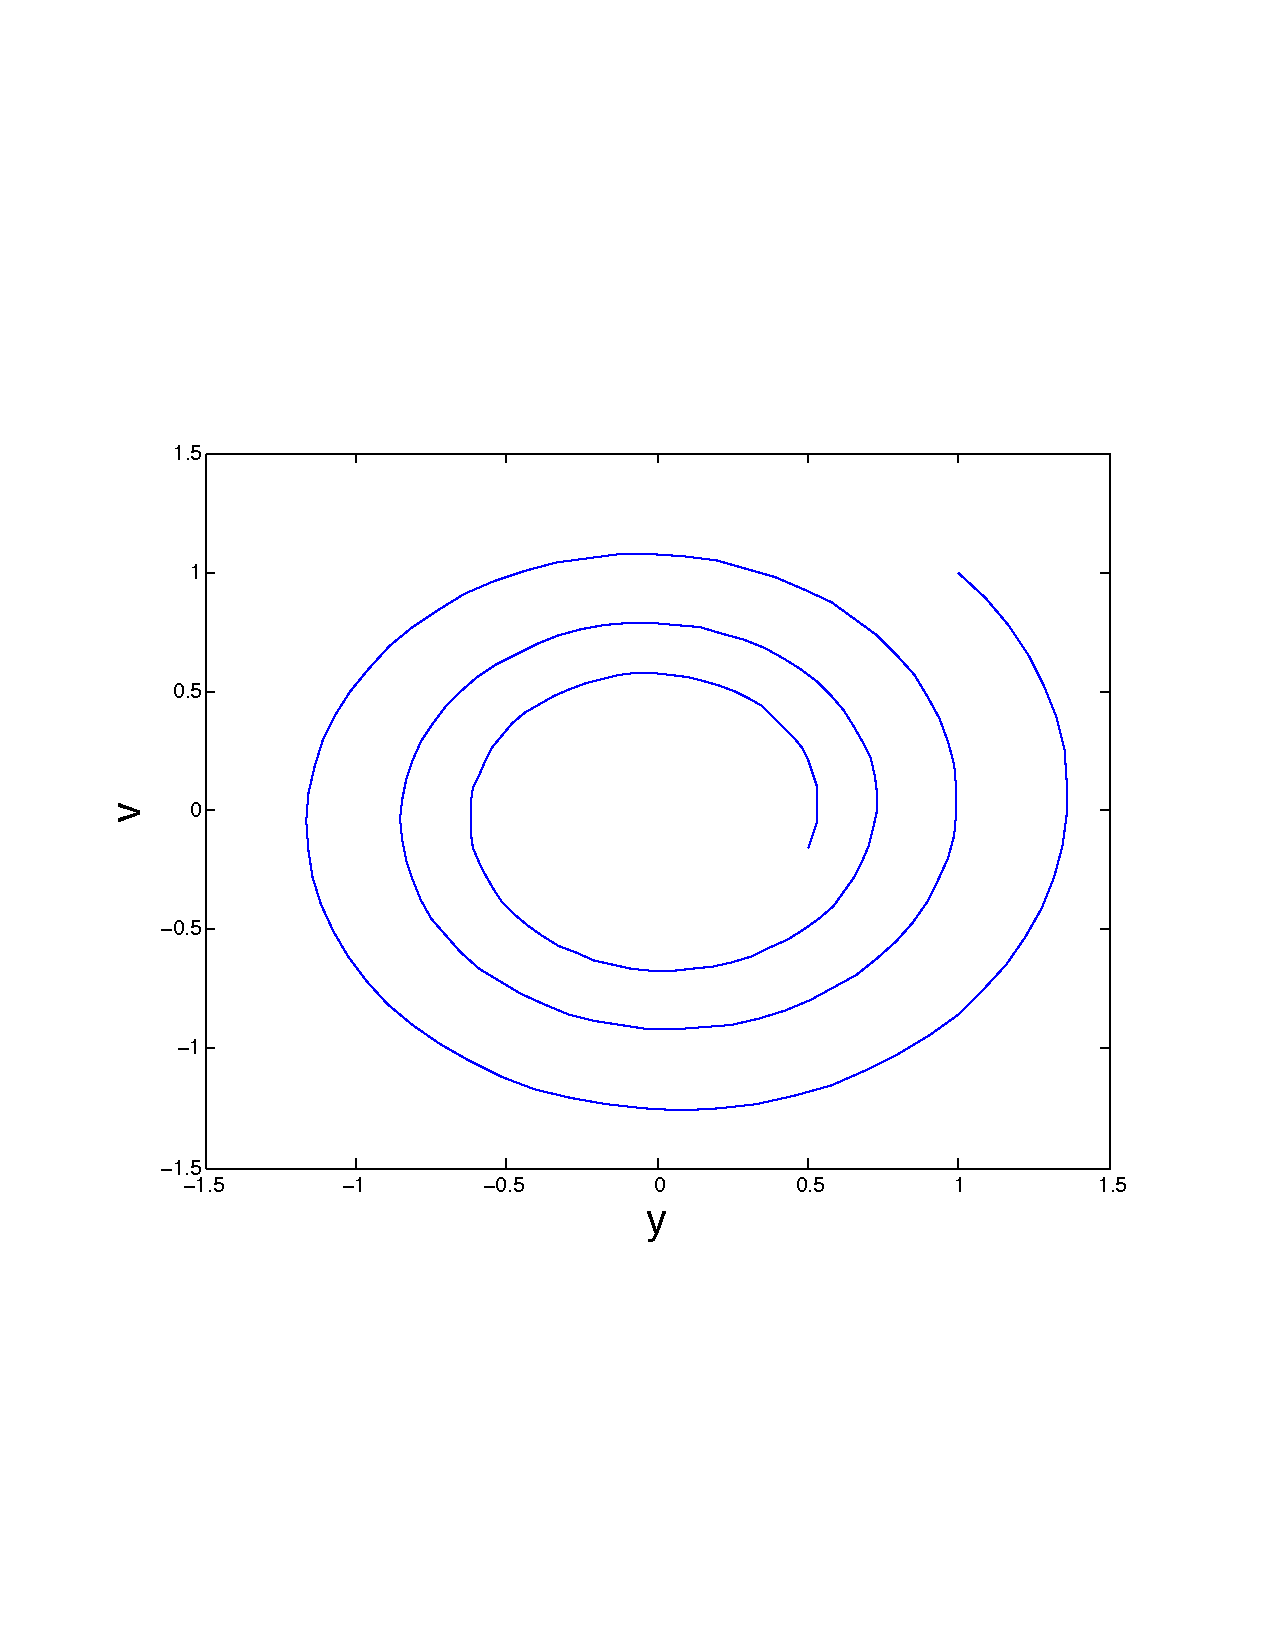
\includegraphics[width=0.5\textwidth]{andy_exam01_prb04_01.pdf}
  \caption{Phase plot of the harmonic oscillator solved with simple implicit Euler method.}
\end{figure}

\lstinputlisting[language=Matlab]{andy_exam01_prb04.m}
\lstinputlisting[language=Matlab]{andy_IE_ho.m}

\item No. In a previous HW assignment, I showed that the stability region of the modified implicit Euler scheme is the left half of the complex plane.
This region is smaller than that for the simple implicit Euler scheme, but still contains the imaginary axis and so I would also expect the solution to decay.
Qualitatively, therefore, the results will be the same.
\end{enumerate}

\end{enumerate}

%% \begin{figure}[h!]
%%   \centering
%%     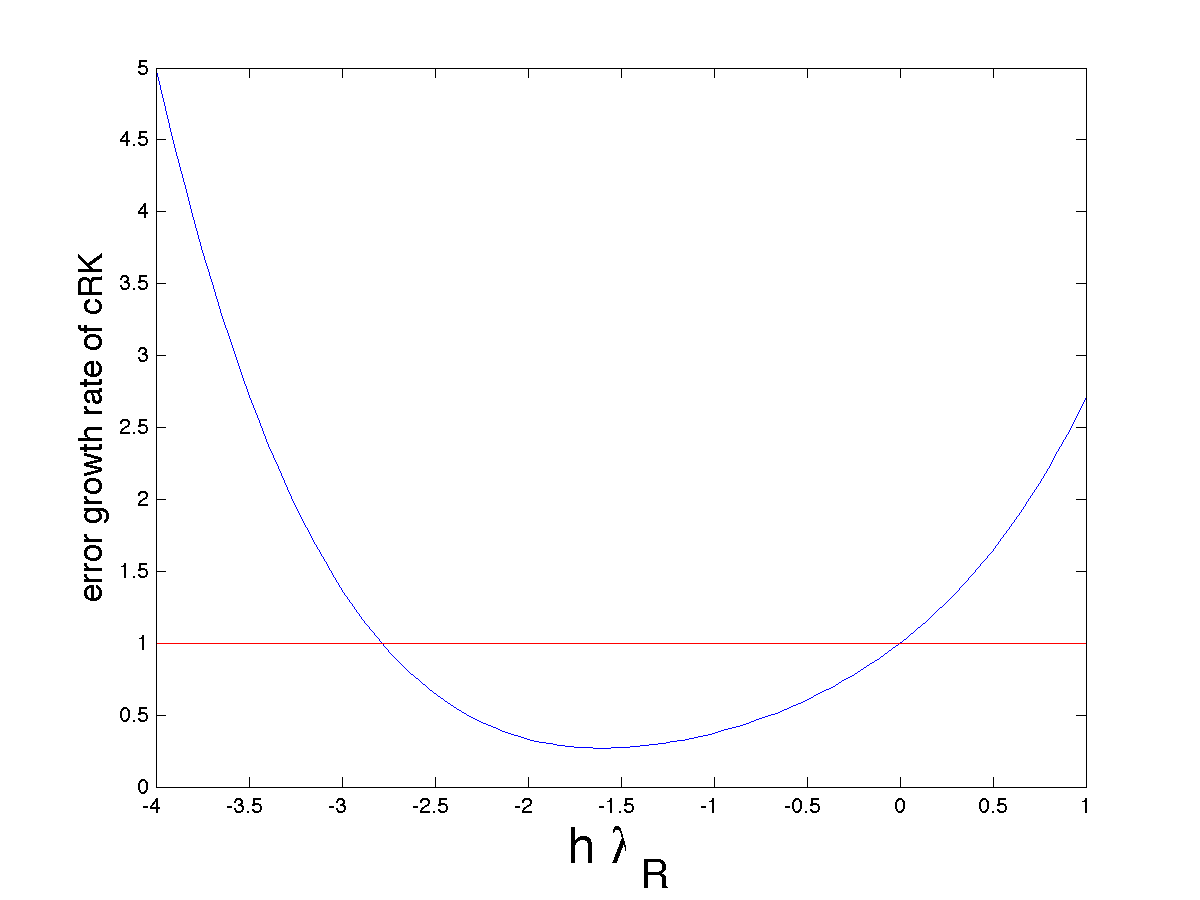
\includegraphics[width=0.5\textwidth]{andy_hw04_prb02_01.png}
%%   \caption{Stability of the cRK method.}
%% \end{figure}

%% \lstinputlisting[language=Matlab]{andy_hw04_prb04.m}

\end{document}
